\documentclass[11pt,a4paper]{article}
\usepackage[T1]{fontenc}
\usepackage[utf8]{inputenc}
\usepackage{lmodern}
\usepackage[margin=27mm,headheight=15pt]{geometry}
\usepackage{amsmath,amssymb,amsthm,mathtools}
\usepackage{booktabs,array,longtable}
\usepackage{microtype,enumitem,fancyhdr}
\usepackage{tikz}
\usetikzlibrary{positioning,calc}
\usepackage{listings}
\usepackage{hyperref}
\usepackage[nameinlink,noabbrev]{cleveref}
\hypersetup{colorlinks=true,linkcolor=black,citecolor=black,urlcolor=blue!45!black,
 pdftitle={Cycle-Envelope Kernels for Disk Completion},
 pdfauthor={Research continuation for ProveIt, prepared with ChatGPT}}
\pagestyle{fancy}\fancyhf{}
\fancyhead[L]{\small Cycle-envelope kernels}
\fancyhead[R]{\small ProveIt research continuation}
\fancyfoot[C]{\thepage}
\setlength{\parskip}{4pt}
\setlength{\parindent}{1.2em}
\setlength{\emergencystretch}{2em}
\setlist{itemsep=3pt,topsep=5pt}
\lstset{basicstyle=\ttfamily\small,columns=fullflexible,keepspaces=true,breaklines=true,frame=single}
\newtheorem{theorem}{Theorem}[section]
\newtheorem{lemma}[theorem]{Lemma}
\newtheorem{proposition}[theorem]{Proposition}
\newtheorem{corollary}[theorem]{Corollary}
\theoremstyle{definition}
\newtheorem{definition}[theorem]{Definition}
\newtheorem{example}[theorem]{Example}
\theoremstyle{remark}
\newtheorem{remark}[theorem]{Remark}
\newcommand{\F}{\mathbb F_2}
\newcommand{\Part}{\operatorname{Part}}
\newcommand{\rk}{\operatorname{rank}}
\newcommand{\comp}{\operatorname{comp}}
\newcommand{\poly}{\operatorname{poly}}
\newcommand{\opt}{\operatorname{opt}}
\newcommand{\one}{\mathbf 1}
\newcommand{\ind}[1]{[\,#1\,]}
\newcommand{\Span}{\operatorname{span}}
\newcommand{\snapshot}{66098968e88bba797143ac1bf7ad0ac4c5f697df}
\newcommand{\SingleDirect}{10.02}
\newcommand{\SingleRoot}{56.66}
\newcommand{\SingleCycle}{36.91}

\title{\textbf{Cycle-Envelope Kernels for Disk Completion}\\[5pt]
\Large Exact $2^\lambda$ compression beyond frontier width\\[6pt]
\large A constructive continuation toward quasi-polynomial unknot recognition}
\author{Research contribution prepared for the ProveIt project\\
\small Mathematical development and reference software prepared with ChatGPT}
\date{9 October 2026}
\begin{document}
\maketitle
\begin{abstract}
Recent ProveIt reports prove an optimal $2^{r-1}$ representative bound on $r$ labelled
boundary arcs when every cap partition is permitted. We strengthen this interface theorem
using certified restrictions on both sides. Let past partitions refine $\sigma$ and future
partitions refine $\rho$. Their bipartite incidence multigraph has one edge per arc. If it
is connected and has cycle rank $\lambda=r+1-|\sigma|-|\rho|$, the restricted
disk-completion matrix has binary rank exactly $2^\lambda$; its grade-$j$ block has rank
$\binom\lambda j$. These bounds are sharp for every connected envelope, even for arbitrary
representative-subset methods. Vertex-splitting equations on the cycle space give an
explicit factorization and independently checkable weighted pruning certificates.

For a supplied finite layered disk-patch grammar, safe envelopes are constructible in
polynomial time by joining all local options. Repeated cycle-basis reduction preserves
minimum-cost successful assemblies. A straightforward algorithm runs in
$\poly(I,B)2^{3\lambda_*}$ bit time, where $I$ is explicit grammar length, $B$ bounds cost
bit lengths, and $\lambda_*$ is maximum envelope cycle rank. The sufficient
quasi-polynomial regime is therefore $\lambda_*=O(\log^2 n)$, not necessarily
$r=O(\log^2 n)$; actual arc counts can remain polynomially large.

The package includes a complete finite-grammar solver, separate pruning and run checkers,
and literal triangulated-surface replay. Forty-two test methods pass. Additional audits
check 633,531 compatibility entries, 1,000 weighted families, 600 three-way grammar
comparisons, and 1,412 fully enumerated assignments. Restricted-envelope benchmarks retain
four candidates instead of 16--29 in the unrestricted basis and improve its measured median
search times by 1.49--3.04 times. Single-cap preprocessing remains slower than direct
scanning. These are abstract-grammar measurements, not native recognizer timings.
No complete low-cycle-envelope producer for all knot exteriors, or general
quasi-polynomial recognition bound, is established here.
\end{abstract}
\noindent\textbf{Status.} Self-contained proofs and executed standalone software. Classical
rank-based and exterior-algebra methods are credited; worldwide priority for equivalent
formulations is not asserted. No proof-assistant verification or native runtime integration
is claimed.
\clearpage
\begingroup\small\setlength{\parskip}{0pt}\tableofcontents\endgroup
\clearpage

\section{Research position and the precise advance}\label{sec:position}
\subsection{The current repository already has a source bridge}
The reviewed ProveIt revision is
\begin{center}\small\texttt{\snapshot}.\end{center}
The maintained \path{Topology/UnknotRecognition} material distinguishes its exact
recognizers from the general quasi-polynomial implementation target \cite{repo}.
The canonical diagram-to-exterior bridge is no longer absent. The inspected source
\path{synthesis/diagram_exterior.tex} constructs and separately checks a compact
knot-exterior triangulation from a validated planar one-component PD code. Its pulling
subdivision has $20\max(1,n)$ tetrahedra and $8\max(1,n)$ boundary triangles for an
$n$-crossing diagram \cite{exterior}. That source theorem is existing infrastructure,
not a result of this delivery.

Recent project reports also describe source-bound normal-surface component analysis and
compressing-disk tests for supplied normal vectors \cite{kernels,signed}. Fast verification
of one binary-encoded normal surface does not by itself construct a complete collection
of candidate surfaces, expose manageable interfaces, or bound all geometric search
choices. Our contribution addresses a search-table parameter after an explicit
surface-assembly language has been supplied.

Lackenby's July 2026 hierarchy paper supplies geometric context. Its Section~9 separates
the number of certain algorithmic steps from a running-time estimate for operations whose
implementation costs are not yet specified there \cite{lackenby}. We do not obtain an
end-to-end bound by treating those operations as unit cost. The conditional application
below charges construction, type information, bit lengths, and witness verification.

\subsection{What the incoming reports already prove}
The incoming \emph{Disk-Completion Kernels} and \emph{Optimal Disc-Completion Bases}
manuscripts establish sharp unrestricted binary rank $2^{r-1}$ and the corresponding
weighted representative bound \cite{kernels,bases}. The signed-continuation manuscript
studies orientation consistency and finite patch selection \cite{signed}. We inspected
Library texts and the incoming archive inventory, but did not unpack and establish byte
identity with every incoming ZIP. The source audit records this limitation.

The unrestricted bound cannot be improved while preserving every cap on $r$ arcs.
That is not the same as saying every actual continuation language requires that many
representatives. A future region may never join certain pairs of arcs. A past region can
have analogous restrictions. We ask:
\begin{quote}
Given certified coarse connectivity envelopes on both sides, what is the exact rank and
representative size for all refinements of those envelopes?
\end{quote}
We answer this for every pair of envelopes. The exponent $r-1$ becomes the cycle rank
of their incidence graph. We also construct safe envelopes from a complete explicit patch
grammar in polynomial time, without first enumerating all suffix states.

\subsection{Established methods and the novelty boundary}
Cost-ordered rank bases for weighted connectivity problems are classical \cite{bckn}.
Exterior-algebra representative families for linear matroids are also established tools
\cite{flps}. Gaussian elimination, the representative replacement argument, and
single-exponential connectivity dynamic programming are not claimed as new.
The overlap dimension of representable subspaces relates to the standard matroid
connectivity function \cite{seymour}; \cref{prop:overlap} makes this explicit here.

The developed contribution is the exact \emph{two-sided disk-completion} theorem, its
sharpness for each connected envelope, the vertex-splitting factorization, the constructive
envelope compiler and composition proof, and an independently checked executable search.
This is an application and refinement of classical methods. An exhaustive worldwide
priority search for every equivalent formulation has not been completed.

\section{Topology and the two-sided interface}\label{sec:topology}
\subsection{The boundary-arc contract}
All local surfaces are compact finite PL surfaces, each component having nonempty boundary.
An attachment arc is a proper closed interval in a boundary circle. Distinct arcs in one
surface are disjoint, including their endpoints, and have disjoint collars. Attachments
glue specified arc pairs by homeomorphisms with no other identifications; corners are
smoothed. The quotient is again a compact surface with boundary.

One label denotes one actual connected interval, not a point-incidence histogram or an
arbitrarily large bundle of parallel intervals. All actual intervals contribute to the
Euler calculation. Ambient positions, boundary framings, quadrilateral restrictions, and
other continuation-visible geometry must be fixed in a separate type. A partition alone
does not certify an embedding in a three-manifold.

Write $c(S)=\comp(S)$ and $\delta(S)=c(S)-\chi(S)$. For a connected orientable
surface of genus $g$ with $h\ge1$ boundary circles, $\delta=2g+h-1$. For a connected
nonorientable surface with $k$ crosscaps and $h\ge1$ boundary circles,
$\delta=k+h-1$. Thus $\delta(S)\ge0$, with equality exactly for disk unions.

\begin{lemma}[Defect under separated boundary-arc attachments]\label{lem:defect}
Glue $r$ arc pairs between surfaces $S,T$ satisfying the contract. Let $G$ have one vertex
per component of either surface and one edge per glued pair, including isolated vertices.
For the quotient $W$,
\begin{align}
 c(W)&=c(G), & \chi(W)&=\chi(S)+\chi(T)-r,\label{eq:chi}\\
 \delta(W)&=\delta(S)+\delta(T)+\beta_1(G), &
 \beta_1(G)&=r-c(S)-c(T)+c(G).\label{eq:defect}
\end{align}
Hence $W$ is a disk union exactly when $S,T$ are disk unions and $G$ is a forest; it
is one disk exactly when the pieces are disk unions and $G$ is a tree.
\end{lemma}
\begin{proof}
Paths between original components cross glued intervals, so quotient connectivity equals
graph connectivity. Triangulate compatibly with the intervals. Each glued interval has
Euler characteristic one; their disjointness excludes higher-intersection corrections.
Inclusion--exclusion gives \eqref{eq:chi}. Substitute into $c(W)-\chi(W)$ to get
\eqref{eq:defect}.

Every original boundary circle has points outside its finitely many disjoint proper
closed attachment intervals. These survive on the quotient boundary. All quotient
components therefore have nonempty boundary. Every term on the right of \eqref{eq:defect}
is nonnegative, and their sum is zero exactly in the stated forest case. The connected
case is the tree case.
\end{proof}

This is the topological mechanism used in the predecessor reports \cite{kernels,bases},
recalled to make this strengthening self-contained. No orientation signs are required for
the disk case: a leaf disk in a tree can always be oriented compatibly with its neighbor.
Positive defect cannot be repaired by later permitted attachments. A nonterminal component
with no live arc cannot join a required nonempty remainder and must be rejected.

\subsection{Partitions and certified envelopes}
Let $U$ be a set of $r\ge1$ labels. For $p,q\in\Part(U)$, write $|p|$ for the number
of blocks, $p\preceq\sigma$ for refinement, and $p\vee q$ for the least common
coarsening. Its blocks are generated by alternating paths within blocks of $p$ and $q$.
A disk-union frontier meeting every live arc determines $p$: two arcs have the same
block exactly when they lie on the same disk.

The bipartite multigraph $G(p,q)$ has a vertex for every block of $p$ or $q$, and an
edge $u\in U$ between its containing blocks. Every vertex meets an edge. Thus
\begin{equation}
 D(p,q)=\ind{p\vee q=\one_U\text{ and }|p|+|q|=r+1}
 \label{eq:disk}
\end{equation}
is exactly the tree indicator, and hence the disk-completion indicator under the arc
contract by \cref{lem:defect}.

\begin{definition}[Two-sided connectivity envelope]\label{def:envelope}
An envelope is a pair $(\sigma,\rho)$ of partitions of $U$. It is safe for a candidate
family and continuation language when every candidate has $p\preceq\sigma$ and every
permitted complementary disk union has $q\preceq\rho$. Its incidence graph is
$H=G(\sigma,\rho)$. The restricted matrix $\mathcal D_{\sigma,\rho}$ has rows all
$p\preceq\sigma$, columns all $q\preceq\rho$, and entries $D(p,q)$.
\end{definition}

A safe envelope can include combinations not simultaneously realizable. It is an
overapproximation. Omitting a possible connectivity relation, in contrast, can make
pruning unsound. Certifying an envelope is separate from checking a row identity.

\begin{proposition}[Disconnected-envelope rejection]\label{prop:disconnected}
If $\sigma\vee\rho\ne\one_U$, then $\mathcal D_{\sigma,\rho}$ is zero.
\end{proposition}
\begin{proof}
For refinements, $p\vee q\preceq\sigma\vee\rho$. The former cannot have one block
when the latter has more than one.
\end{proof}
Henceforth suppose $H$ is connected and put
\begin{equation}
 s=|\sigma|,\qquad t=|\rho|,\qquad
 \lambda=\beta_1(H)=r+1-s-t\ge0.
 \label{eq:lambda}
\end{equation}
Parallel-edge multiplicity matters: $a$ parallel arc edges between two vertices contribute
$a-1$ independent cycles, not zero.

\begin{figure}[htbp]
\centering
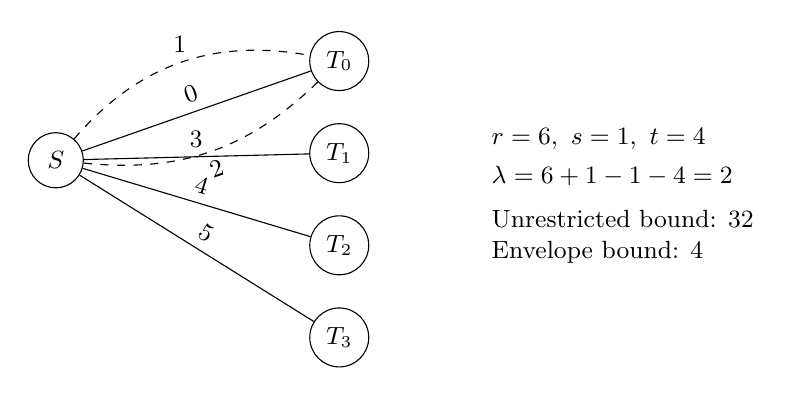
\begin{tikzpicture}[scale=.9,every node/.style={font=\small}]
\node[circle,draw,minimum size=7mm] (s) at (0,0) {$S$};
\node[circle,draw,minimum size=7mm] (t0) at (4,1.4) {$T_0$};
\node[circle,draw,minimum size=7mm] (t1) at (4,.1) {$T_1$};
\node[circle,draw,minimum size=7mm] (t2) at (4,-1.2) {$T_2$};
\node[circle,draw,minimum size=7mm] (t3) at (4,-2.5) {$T_3$};
\draw (s) -- node[above,sloped] {$0$} (t0);
\draw[dashed] (s) to[bend left=30] node[above] {$1$} (t0);
\draw[dashed] (s) to[bend right=25] node[below,sloped] {$2$} (t0);
\draw (s) -- node[above,sloped] {$3$} (t1);
\draw (s) -- node[above,sloped] {$4$} (t2);
\draw (s) -- node[above,sloped] {$5$} (t3);
\node[align=left] at (8,-.5) {$r=6,\ s=1,\ t=4$\\[3pt]
$\lambda=6+1-1-4=2$\\[5pt]Unrestricted bound: $32$\\Envelope bound: $4$};
\end{tikzpicture}
\caption{Two independent cycles. Solid edges form a spanning tree and dashed edges are
chords. Adding pendant arc edges increases $r$ without increasing $\lambda$. All edges
remain genuine arcs; none is silently bundled.}\label{fig:envelope}
\end{figure}

\section{Cycle-space factorization and exact ranks}\label{sec:rank}
\subsection{Vertex splitting as a system of cycle constraints}
The cycle space $Z(H)\subseteq\F^U$ consists of edge vectors with even incidence at
every vertex. It has dimension $\lambda$. Fix a basis $z_1,\ldots,z_\lambda$ and
identify $x\in\F^\lambda$ with $z(x)=\sum_i x_i z_i$.
A refinement $p\preceq\sigma$ splits each $\sigma$-vertex into its $p$-subblocks.
Choose one omitted subblock at every coarse vertex. For every other subblock $C$, impose
\begin{equation}
 \ell_C(x)=\sum_{u\in C}z(x)_u,\qquad
 A_p(C,i)=\sum_{u\in C}z_i(u)\in\F.
 \label{eq:constraints}
\end{equation}
The matrix $A_p$ has $j(p)=|p|-s$ rows and $\lambda$ columns.
Define $B_q$ similarly on the $\rho$-side, with $k(q)=|q|-t$ rows.

\begin{lemma}[Split cycle-space identity]\label{lem:split}
Under the common edge-label identification,
\begin{equation}
 Z(G(p,q))=\left\{z(x):\begin{pmatrix}A_p\\ B_q\end{pmatrix}x=0\right\},
 \qquad
 \beta_1(G(p,q))=\lambda-\rk_{\F}\begin{pmatrix}A_p\\ B_q\end{pmatrix}.
 \label{eq:split}
\end{equation}
\end{lemma}
\begin{proof}
Even incidence at every split vertex implies even incidence at the original vertex by
summing its subblock equations. Hence every split-graph cycle vector lies in $Z(H)$.
Conversely, a vector in $Z(H)$ satisfies the parity equation at each original vertex.
The sum of all its subblock equations is therefore zero. Imposing all but the omitted
equation forces the omitted one too. This holds at each left and right vertex. The
remaining equations are exactly the displayed stacked system. The cycle-basis coordinate
map is an isomorphism, so rank--nullity gives the dimension identity.
\end{proof}

No independence of the remaining equations is assumed. Splitting can disconnect the graph;
then the constraints can be dependent and determinant-zero rows arise naturally.

\begin{lemma}[Determinantal disk predicate]\label{lem:det}
If $j(p)+k(q)=\lambda$, then
\begin{equation}
              D(p,q)=\det_{\F}\begin{pmatrix}A_p\\ B_q\end{pmatrix}.
 \label{eq:det}
\end{equation}
If $j(p)+k(q)\ne\lambda$, then $D(p,q)=0$.
\end{lemma}
\begin{proof}
The split graph has $r$ edges and $s+t+j(p)+k(q)$ vertices. The tree edge--vertex
condition is equivalent to $j(p)+k(q)=r+1-s-t=\lambda$. If it fails, the disk predicate
is zero. If it holds, the graph has $r+1$ vertices. A graph with $r$ edges and $r+1$
vertices is a tree exactly when its cycle space is zero: a forest with these counts has
one component. By \cref{lem:split}, this is equivalent to nonsingularity of the square
stacked matrix. Over $\F$ the determinant is zero or one. The empty $0\times0$
determinant is one, which includes $\lambda=0$.
\end{proof}

\subsection{Explicit exterior coordinates}
Let $[\lambda]=\{1,\ldots,\lambda\}$, with $[0]=\varnothing$. For every
$J\subseteq[\lambda]$, define
\begin{equation}
 F_\sigma(p,J)=
 \begin{cases}\det A_p[:,J],& |J|=j(p),\\0,&|J|\ne j(p).\end{cases}
 \label{eq:feature}
\end{equation}
If $j(p)>\lambda$, the whole row is zero. Define $F_\rho$ using $B_q$, and let
$\mathcal J$ be the permutation matrix of $J\mapsto[\lambda]\setminus J$.

\begin{theorem}[Cycle-envelope factorization]\label{thm:factor}
Over $\F$,
\begin{equation}
              \mathcal D_{\sigma,\rho}=F_\sigma\mathcal JF_\rho^{\mathsf T}.
 \label{eq:factor}
\end{equation}
The feature dimension is $2^\lambda$, and rows of grade $j(p)$ are supported in a
coordinate space of dimension $\binom\lambda{j(p)}$.
\end{theorem}
\begin{proof}
For noncomplementary grades, no subset has size $j(p)$ while its complement has size
$k(q)$, so the pairing is zero. For complementary grades, Laplace expansion of the
stacked determinant by its first $j(p)$ rows gives
\[
 \det\begin{pmatrix}A_p\\B_q\end{pmatrix}
 =\sum_{\substack{J\subseteq[\lambda]\\ |J|=j(p)}}
          \det A_p[:,J]\det B_q[:,[\lambda]\setminus J].
\]
All signs disappear in characteristic two. Apply \cref{lem:det}. Homogeneous support
in \eqref{eq:feature} gives the graded dimension.
\end{proof}

\begin{proposition}[Exactly which rows vanish]\label{prop:zero}
For $p\preceq\sigma$, put $a=c(G(p,\rho))=|p\vee\rho|$. Then
\begin{equation}
                         \rk A_p=j(p)-a+1.
 \label{eq:rankA}
\end{equation}
Consequently $F_\sigma(p,\cdot)\ne0$ exactly when $p\vee\rho=\one_U$.
\end{proposition}
\begin{proof}
Use \cref{lem:split} with $q=\rho$, so there are no right-side constraints. The cycle
rank of that graph is
$r-(|p|+t)+a=\lambda-j(p)+a-1$.
Subtracting from $\lambda$ proves \eqref{eq:rankA}. A matrix with $j(p)$ rows has a
nonzero maximal minor exactly when it has row rank $j(p)$, including the empty-row case.
Thus a nonzero feature is equivalent to $a=1$.
\end{proof}

This provides a cheap connectivity prefilter before feature construction. The delivered
unrestricted-root and exact-state comparators receive this same prefilter; the measured
improvement is not obtained by withholding an obvious rejection rule.

\subsection{Sharpness for every connected envelope}
Choose a spanning tree $T$ of $H$, with chords $e_1,\ldots,e_\lambda$. Their fundamental
cycle basis satisfies $z_i(e_j)=\ind{i=j}$. Every original vertex has a tree edge.
For $S\subseteq[\lambda]$, construct $p_S\preceq\sigma$ by detaching the left
endpoint of each chord indexed by $S$ into a singleton subblock. All other incident
labels stay in a core subblock, which is nonempty because it retains a tree edge.
Similarly define $q_R\preceq\rho$ by detaching right endpoints indexed by $R$.

\begin{lemma}[Chord-detachment witnesses]\label{lem:chord}
With core subblocks omitted in the feature construction,
\[
 F_\sigma(p_S,\cdot)=e_S,\qquad F_\rho(q_R,\cdot)=e_R.
\]
Independently of coordinate choices,
\begin{equation}
                      D(p_S,q_R)=\ind{R=[\lambda]\setminus S}.
 \label{eq:permutation}
\end{equation}
\end{lemma}
\begin{proof}
A detached singleton chord imposes the coordinate equation $x_i=0$, giving the stated
unit exterior vector. For a direct graph proof, a chord detached at both ends becomes
a separate component while the core spanning tree remains. If the detachment sets are
disjoint but do not cover all chords, their total size is less than $\lambda$, so the
tree edge--vertex count fails. If they partition the chords, the core is $T$ and each
former chord is now a pendant edge attached at its undetached endpoint. The result is
a tree.
\end{proof}

\begin{theorem}[Exact total and graded ranks]\label{thm:rank}
For every connected envelope,
\begin{equation}
                 \rk_{\F}\mathcal D_{\sigma,\rho}=2^\lambda.
 \label{eq:exactrank}
\end{equation}
The block with $|p|=s+j$ and $|q|=t+\lambda-j$ has exact rank
$\binom\lambda j$ for $0\le j\le\lambda$.
\end{theorem}
\begin{proof}
The factorization gives both upper bounds. The rows $p_S$ and columns $q_R$ form a
subset-complement permutation matrix of order $2^\lambda$. Restricting to $|S|=j$
and $R=[\lambda]\setminus S$ gives a permutation submatrix of order $\binom\lambda j$
in that grading. These lower bounds match the upper bounds. When $\lambda=0$, the
single distinguished entry is $D(\sigma,\rho)=1$.
\end{proof}

This is a binary-rank statement, not a claim about all field characteristics. The sharp
families are realizable as abstract polygonal disk unions with separated labelled arcs.
Simultaneous realization in one embedded knot-region type remains a geometric question.

\subsection{Cycle rank as a representable overlap parameter}
\begin{proposition}[Linear-matroid interpretation]\label{prop:overlap}
For a partition $\tau$, let
\[
 V_\tau=\Span_{\F}\{e_u+e_v:u,v\text{ belong to one block of }\tau\}\subseteq\F^U.
\]
Then $\dim V_\tau=r-|\tau|$, and for a connected envelope,
\begin{equation}
                 Z(H)=V_\sigma\cap V_\rho,\qquad
                 \dim(V_\sigma\cap V_\rho)=\lambda.
 \label{eq:overlap}
\end{equation}
\end{proposition}
\begin{proof}
In a block $C$, the differences from one fixed element to the others form a basis of
vectors with even coordinate sum on $C$. Hence $V_\tau$ is exactly the space of vectors
having even sum on every $\tau$-block, of dimension $\sum_C(|C|-1)=r-|\tau|$.
The simultaneous parity conditions for $\sigma$ and $\rho$ are exactly those of
$Z(H)$. Alternatively, $V_\sigma+V_\rho=V_{\sigma\vee\rho}$ because differences
propagate along join paths. The connected join has dimension $r-1$, and the intersection
dimension formula gives $r+1-s-t$.
\end{proof}

Taking separately colored spanning forests inside the $\sigma$- and $\rho$-blocks gives
a graphic-matroid interpretation: their rank sum minus the rank of their union is
$\lambda$. This relates the parameter to established connectivity and representative-set
methods \cite{seymour,flps}; the factorization here makes its disk-specific behavior explicit.

\section{Weighted representatives and independently checked pruning}\label{sec:weighted}
\subsection{The optimization guarantee}
A candidate $a$ consists of an actual partial-surface witness, its partition $p_a$, and an
integer cost $w_a$ written in binary. All candidates in one reduction call have a fixed
geometric type. For a finite family $\mathcal A$ and $q\preceq\rho$, put
\[
 \opt(\mathcal A,q)=\min\{w_a:a\in\mathcal A,\ D(p_a,q)=1\},
 \qquad \min\varnothing=+\infty.
\]
A subset represents $\mathcal A$ when it preserves this optimum for every such $q$.
Costs may be negative, since the candidate family and assembly language are finite.

\begin{theorem}[Optimal cycle-envelope representative bound]\label{thm:weighted}
If every $p_a\preceq\sigma$ and the envelope is connected, a deterministic algorithm
retains a representative subset $\mathcal A'$ of original candidates satisfying
\begin{equation}
 |\mathcal A'|\le2^\lambda,\qquad
 |\{a\in\mathcal A':|p_a|=s+j\}|\le\binom\lambda j.
 \label{eq:weightedbound}
\end{equation}
It scans in nondecreasing cost and retains a candidate exactly when its feature row is
independent of previously retained rows. Zero rows are discarded.
\end{theorem}
\begin{proof}
Fix a total order refining cost order. Gaussian elimination retains an independent
family; homogeneous support in \cref{thm:factor} gives the size bounds. Every discarded
row has an expansion
\begin{equation}
 F_\sigma(p_a,\cdot)=\sum_{b\in E_a}F_\sigma(p_b,\cdot),\qquad
 b\in\mathcal A',\quad w_b\le w_a.
 \label{eq:expansion}
\end{equation}
For any cap completing $a$, pair this identity with
$\mathcal JF_\rho(q,\cdot)^{\mathsf T}$. The left side is one, so at least one summand
is one. A retained candidate of no greater cost therefore completes that same cap.
Apply this to an optimum candidate. The reverse inequality holds because the retained
family is a subset. Infeasibility is preserved for the same reason.
\end{proof}

The parity calculation finds a replacement for each particular successful row; it is
not a randomized parity-of-solutions decision. A retained row refers to an original
witness, not an XOR of surfaces.

\begin{theorem}[Sharpness for all representative-subset methods]\label{thm:lower}
For every connected envelope there is a cost-zero family requiring all $2^\lambda$
representatives to preserve every allowed cap query. In grade $j$ there is such a family
requiring all $\binom\lambda j$ candidates.
\end{theorem}
\begin{proof}
Take one candidate for every $p_S$ in \cref{lem:chord}. The cap
$q_{[\lambda]\setminus S}$ completes exactly that candidate among the family.
Omitting it changes its query from feasible to infeasible. Restrict to $|S|=j$ for
the graded statement.
\end{proof}

This is not a running-time lower bound for arbitrary algorithms. One explicitly supplied
cap can be checked against an explicit candidate list by a direct polynomial-time scan;
no exponential-dimensional preprocessing is necessary for that isolated task.

\subsection{Sectors, coordinate changes, and certificates}
Suppose an auxiliary label lies in $Q$ sectors and the continuation condition determines
the required sector independently of internal partition. Reduction separately in each
sector preserves the corresponding queries and uses at most $Q2^\lambda$ candidates.
The implementation uses two-bit sectors with XOR composition, so $Q\le4$. They are
actual boundary-homology sectors only under the geometric chain contract in
\cref{sec:integration}.

A pruning certificate lists retained original indices and an expansion
\eqref{eq:expansion} for every source row. It binds the ordered source partitions, costs,
sectors, witnesses, and envelopes. The checker reconstructs the feature rows, verifies
each expansion, checks cost and sector constraints, and checks the graded size bounds.
Independence helps produce a small family, but these expansion identities and cost
inequalities suffice to certify representativity.

\begin{proposition}[Coordinate independence of pruning identities]\label{prop:invariance}
Changing the cycle-space basis or the omitted subblock at any coarse vertex leaves the
validity of homogeneous linear expansion identities unchanged.
\end{proposition}
\begin{proof}
A cycle-basis change right-multiplies every constraint matrix by one fixed invertible
matrix. Its action on degree-$j$ maximal minors is the invertible map on the $j$th
exterior power. Linear identities in that grade are therefore preserved.

At a coarse vertex, the sum of all subblock parity rows is zero. Changing the omitted
subblock changes its $m-1$ listed rows by an invertible linear combination. The determinant
of that transformation over $\F$ is one. Row permutations also have determinant one.
Thus the wedge of all constraint rows, and all its maximal minors, is unchanged, even
when the evaluated rows are dependent. Different grades have disjoint coordinate supports,
so identities decompose by grade.
\end{proof}

The producer computes fundamental cycles and sparse exterior products. The checker
instead obtains a cycle basis by row-reduced nullspace elimination and computes features
by enumerating square minors. It omits the last subblock instead of the first.
\Cref{prop:invariance} justifies these genuinely different coordinate choices.

A SHA-256 digest is convenient source binding, not a proof by itself. The checker receives
the actual ordered source family independently and reconstructs the payload. A valid row
certificate still does not prove that the supplied envelopes cover every geometric
continuation. That is a separate compiler or producer assertion.

\subsection{Encoded local cost}\label{sub:localcost}
Let $L$ be the supplied candidate count, $B$ the maximum cost bit length, and $W$ their
explicit witness encoding length. Put $d=2^\lambda$. A spanning tree and fundamental
cycles are constructed in polynomial time in $r,\lambda$. A feature can be computed by
sparse exterior multiplication in $\poly(r,\lambda)d$ bit work. Alternatively, enumerate
its $\binom\lambda j$ square minors using binary elimination, giving the same
single-exponential form with a different polynomial.

Naive elimination uses at most $d$ pivots per row and XORs $d$-bit vectors. Tracking
expansions into retained rows costs the same order. Thus a conservative local bound is
\begin{equation}
 \poly(r,\lambda)+O\!\left(Ld^2+L\poly(r,\lambda)d
                    +LB\log(L+1)+W\right),
 \label{eq:localcost}
\end{equation}
with additional polynomial charges for source encoding. The independent checker can
use the same $Ld^2$ expansion bound and $L\poly(r,\lambda)d$ minor-construction bound.

The basis and its binary expansions occupy $O(d^2)$ bits. An explicit certificate with
at most $d$ indices per input row uses $O(Ld\log(L+1))$ bits. Source candidates and
witnesses remain additional storage. A $d$-bit packed-integer XOR is charged $O(d)$ bit
operations, not treated as constant time. There is no pseudo-polynomial dependence on
the numerical values of the costs.

An explicitly Bell-sized input family must still be read. The next section turns this
family-level reduction into a search theorem by generating later candidates only from
already reduced families and an explicit finite option set.

\section{A complete finite grammar and polynomial envelope compiler}\label{sec:grammar}
\subsection{The supplied language}
Fix nonempty interfaces $U_0,\ldots,U_h$ with $r_i=|U_i|$. A layered grammar supplies an
explicit initial family of disk unions on $U_0$; for each $i=1,\ldots,h$, an explicit
list of disk-union patches on $U_{i-1}\sqcup U_i$; and an explicit family of disk-union
caps on $U_h$. Choose one initial object, one option at every layer, and one cap.
Costs add and sectors XOR. Matching incoming and outgoing arc labels are glued.
Terminal success is one disk with an allowed final sector.

Every local option is available independently of the current partition. Topological
checks reject attachment cycles or sealed components, but there are no hidden
same-component guards. For an ambient application, sufficient geometric types must
ensure that the same outside objects and arc maps are legal for every candidate of the
type. Boundary or embedding information visible to the continuation belongs in that type.

The reference solver is complete for this explicit abstract language, not automatically
for disks in a knot exterior. Its result names are deliberately
\begin{quote}\ttfamily
FOUND\_ABSTRACT\_DISK\qquad NO\_DISK\_IN\_GRAMMAR.
\end{quote}
Neither is automatically an unknot or knottedness verdict.

\subsection{Forward and backward envelope recurrences}
For disjoint sets, $\alpha\oplus\operatorname{disc}(V)$ denotes the partition equal to
$\alpha$ on one set and discrete on $V$. Restriction followed by canonical relabelling
is denoted $\tau|_V$. Write $\mathcal P_i$ for the layer-$i$ partitions and $\mathcal C$
for the cap list. Define
\begin{align}
 \sigma_0&=\bigvee_{a\in\mathcal A_0}p_a,\label{eq:forward0}\\
 \sigma_i&=\left((\sigma_{i-1}\oplus\operatorname{disc}(U_i))
            \vee\bigvee_{\pi\in\mathcal P_i}\pi\right)\big|_{U_i},
            &&1\le i\le h,\label{eq:forward}\\
 \rho_h&=\bigvee_{q\in\mathcal C}q,\label{eq:back0}\\
 \rho_{i-1}&=\left((\operatorname{disc}(U_{i-1})\oplus\rho_i)
            \vee\bigvee_{\pi\in\mathcal P_i}\pi\right)\big|_{U_{i-1}},
            &&h\ge i\ge1.\label{eq:backward}
\end{align}
The join of an empty option list is discrete on its specified label set. Empty languages
are allowed and yield no success.

\begin{theorem}[Constructive safe envelopes]\label{thm:compiler}
Every realizable prefix partition at $U_i$ refines $\sigma_i$, and every realizable
complementary suffix partition meeting $U_i$ refines $\rho_i$. Both sequences are
computable in polynomial time in the explicit grammar length, without enumerating
prefix or suffix assemblies.
\end{theorem}
\begin{proof}
The initial statement follows from \eqref{eq:forward0}. Suppose a prefix partition $p$
refines $\sigma_{i-1}$. For a chosen patch $\pi$, quotient connectivity on outgoing arcs
is the restriction of $(p\oplus\operatorname{disc}(U_i))\vee\pi$.
Join and restriction preserve refinement. Replacing $p$ by $\sigma_{i-1}$ and $\pi$
by the join of every option only coarsens that partition. This proves the forward induction.
The suffix induction is identical in reverse order, starting from the cap family.

Each join connects labels in every explicitly listed block. Disjoint-set union or graph
connectivity computes it in polynomial time in the listed incidences. No Cartesian-product
candidate family is generated. Repeating over all layers is polynomial in input length.
\end{proof}

The compiler joins mutually exclusive options. This may create impossible connections
and overestimate $\lambda_i$, losing compression but not correctness. Computing the
smallest envelope of all realizable successful contexts is a different problem and is
not silently assumed solved.

The independent checker uses a universal graph on all interface labels, not the recursive
disjoint-set compiler. It separately takes whole-prefix and whole-suffix connectivity
and restricts to each cut. Both constructions express the transitive closure of the
same local block relations; their equality is also checked on randomized grammars.

\subsection{Transitions and context-safe replacement}
To attach a current disk union to a patch, form their component-incidence graph with one
edge per incoming arc. Reject an attachment cycle. Otherwise its graph components are
disks by \cref{lem:defect}. Reject any component with no outgoing arc, since nonempty
later material must still join the final disk. Restrict surviving component labels to
outgoing arcs to obtain the next partition. A patch component having only outgoing arcs
is allowed: it is a new disk, initially an isolated vertex in this attachment graph.

Identical partition/sector states can first be deduplicated by keeping the cheapest
witness. Every solver mode uses the same deterministic deduplication, transition generator,
and safe filter $p\vee\rho_i=\one_{U_i}$. Cycle mode then applies the representative
theorem to $(\sigma_i,\rho_i)$.

\begin{theorem}[Context-safe cycle-envelope replacement]\label{thm:composition}
Replacing an interface family by representatives for its safe two-sided envelope preserves
the minimum cost of every successful terminal assembly. Repeated replacements throughout
the supplied grammar preserve global minimum cost and feasibility.
\end{theorem}
\begin{proof}
Fix a successful complete assembly using a candidate $S$ at the replaced interface.
Glue all pieces outside $S$ according to the selected completion to obtain $T$.
Its entire contact with $S$ is the labelled interface of separated arcs. Since the final
surface is a disk, \cref{lem:defect} makes both $S,T$ disk unions with a tree attachment
graph. Every component of $T$ meets the interface, or the final assembly would be
disconnected. Its cap partition $q$ therefore exists, and the compiler theorem gives
$q\preceq\rho_i$.

Representativity supplies an actual retained $S'$ of the same type and sector, of no
greater cost, completed by that same $q$. All remaining options and arc maps stay legal
because there is no unrecorded partition-dependent guard; in an ambient application this
is the geometric type-substitution contract. The union $S'\cup T$ is a disk.
Its intermediate surfaces cannot have positive defect, since such defect cannot later
disappear. Nor can they have a sealed component followed by nonempty material.
Thus the replacement path survives every local transition and liveness test.

Cost additivity preserves or improves total cost. Conversely a retained subset cannot
introduce an assembly not previously present. Apply this argument successively in the
finite evaluation order to obtain equality of global optima.
\end{proof}

This proof concerns whole remaining contexts, not identical behavior under each individual
next operation. Different caps may use different retained replacements for one discarded
candidate. That is why representatives can be much fewer than physical-state equivalence
classes.

\subsection{The complete run certificate}
A run certificate binds the grammar and supplies one pruning certificate at each interface,
the final optimum, original option indices, and work counters. The checker reconstructs
source candidate lists itself: it tries every supplied option on every previously retained
candidate using an independent breadth-first component-graph transition, performs the
specified cheapest-state deduplication, and checks the reduction certificate against that
reconstructed list. It does not trust a producer's alleged list of generated candidates.
At the end it evaluates every cap query directly.

This validates positive and negative answers \emph{inside the finite grammar}. Omitting an
option from the certificate cannot justify an empty table, because options are independently
read from the source grammar. It does not prove that a geometric producer listed every
patch needed in a knot exterior. That completeness obligation lies outside the language
being checked.

Independent PL replay then expands the selected disks into triangulated polygons, glues
marked boundary edges, checks edge incidences and vertex links, and computes components,
Euler characteristic, boundary circles, and orientability. This is more than repeating
the partition predicate, but still proves abstract topology rather than ambient embedding.

\section{Bit complexity, large interfaces, and adaptive restrictions}\label{sec:complexity}
\subsection{End-to-end accounting for the supplied grammar}
Let $I\ge2$ be the explicit structural bit length, including all partition lists, interfaces,
option indices, sectors, and source data. Let $B\ge1$ bound input cost bit lengths.
Accumulated costs have $O(B+\log(h+2))$ bits. Let $K_i$ be the number of layer-$i$
options and $L_0$ the initial candidate count. These structural quantities and total raw
arc count are charged to $I$.

A disconnected envelope certifies no disk in the supplied grammar by
\cref{prop:disconnected}. Otherwise put
\[
 \lambda_i=r_i+1-|\sigma_i|-|\rho_i|,\qquad
 \lambda_* =\max_{0\le i\le h}\lambda_i.
\]
Let $Q\le4$ be the sector count. More general finite type sets are additional explicit
parameters, not hidden constants.

\begin{theorem}[Cycle-envelope parameterized search]\label{thm:complexity}
The supplied layered grammar can be optimized deterministically, with source-bound
pruning certificates and recovered witnesses, in
\begin{equation}
                            \poly(I,B)2^{3\lambda_*}
 \label{eq:time}
\end{equation}
bit time. The same form bounds checking the run certificate and expanded witness.
The reference implementation satisfies this bound up to polynomial factors when its
allocation guards are disabled or not reached.
\end{theorem}
\begin{proof}
Compile envelopes in polynomial time. Constructing all cycle bases costs polynomial work
in the explicit arc counts. Initial reduction costs $\poly(I,B)4^{\lambda_0}$, charging
$L_0\le I$, by \eqref{eq:localcost}.

At layer $i$, at most $Q2^{\lambda_{i-1}}$ candidates enter. Trying every $K_i$ option
produces at most $K_iQ2^{\lambda_{i-1}}$ transitions. Connectivity, liveness,
canonicalization, arithmetic, and explicit witness-path copying cost polynomial work in
$I,B$ per transition. Output reduction costs at most
\[
                    \poly(I,B)K_iQ2^{\lambda_{i-1}+2\lambda_i}.
\]
Deduplication and sorting add polynomial factors: the logarithm of the generated family
size is $O(\log I+\lambda_*)$, and $\lambda_*\le I$. Summing gives the more detailed
bound
\begin{equation}
 \poly(I,B)\left(L_0 4^{\lambda_0}
       +\sum_{i=1}^{h}K_iQ2^{\lambda_{i-1}+2\lambda_i}
       +Q|\mathcal C|2^{\lambda_h}+1\right),
 \label{eq:nonuniform}
\end{equation}
which implies \eqref{eq:time}. Displaying structural quantities outside the polynomial
here exposes the nonuniform exponent profile; initial-list reading is still charged.

The checker reconstructs the same number of transitions. Its independent minor and
expansion calculations satisfy the same single-exponential local bound. Witnesses select
one explicitly listed patch at each layer, so their polygonal expansion has polynomial
size in $I$. Vertex-link and surface computations are polynomial in that expanded size.
Correctness follows from context-safe replacement and the final direct cap check.
\end{proof}

This deliberately elementary bound uses neither fast matrix multiplication nor optimized
representative-product algorithms. A supplied binary assembly grammar also admits a
$2^{O(\lambda_*)}$ argument by combining two reduced child tables, provided every node
has certified envelopes for its whole context and explicitly bounded type/rule costs.
The executable compiler and full run checker here implement only the layered case.

Keeping all stage certificates costs at most $\poly(I,B)4^{\lambda_*}$ bits under this
accounting, in addition to explicit source storage. Streaming could reduce history but is
not the delivered storage policy. A binary-compressed syntax describing exponentially many
unexpanded options is not an explicit polynomial-size grammar by fiat.

\subsection{Unbounded raw width at fixed cycle rank}
\begin{corollary}[Tree appendages cost no exponential dimension]\label{cor:wide}
Appending arbitrarily many pendant edges with new endpoints to a connected envelope,
or subdividing an edge by an odd-length path to preserve the bipartite sides, leaves
$\lambda$ unchanged. The exact restricted rank stays $2^\lambda$, while the genuine
arc count can grow arbitrarily.
\end{corollary}
\begin{proof}
A pendant edge adds one vertex and one edge and preserves connectivity. Subdivision adds
equal numbers of edges and vertices. Thus $|E|-|V|+1$ is unchanged. Any bipartite graph
without isolated vertices is the incidence graph of the partitions of its edge labels
by left and right endpoints. Apply the exact-rank theorem to these partitions.
\end{proof}

For example, use one left vertex, $\lambda+1$ parallel edges to one right vertex, and
$r-\lambda-1$ additional pendant right vertices. Then
\[
 \sigma=(0,\ldots,0),\qquad
 \rho=(\underbrace{0,\ldots,0}_{\lambda+1},1,2,\ldots,r-\lambda-1).
\]
The exact rank is $2^\lambda$ for every $r\ge\lambda+1$.
The wide-interface test uses $r=256$, $\lambda=3$, and eight sharp chord-detachment
candidates. Producer and independent checker operate on eight-dimensional features,
not $2^{255}$-dimensional features. All 256 arcs remain explicitly represented and read.

\subsection{Narrowing is safe; widening is not}
\begin{proposition}[Monotone restriction of the context language]\label{prop:monotone}
A family representative for all caps refining $\rho$ remains representative when that
allowed cap set is restricted. If safe envelopes are replaced by refinements
$\sigma'\preceq\sigma$, $\rho'\preceq\rho$ and the new incidence graph stays connected,
then
\[
                  \lambda'=r+1-|\sigma'|-|\rho'|\le\lambda.
\]
A new reduction can use this no-larger dimension on candidates still refining the new
past envelope. Widening the future language has no analogous guarantee.
\end{proposition}
\begin{proof}
Equality of optimum functions on a set of queries implies equality on a subset.
Refinement increases block counts, proving the displayed inequality; apply the
representative theorem to the new envelope. The following example proves the last claim.
\end{proof}

For two arcs, take $\sigma=00$, old $\rho=01$, hence $\lambda=0$. Candidates $00$ of
cost zero and $01$ of cost one reduce to only $00$. The newly allowed cap $00$ completes
$01$ but not $00$. An adaptive algorithm widening future options must return to an
unpruned source or have retained representatives for an envelope already containing the
larger language. A resource limit cannot establish that omitted future options are impossible.

Restricting \emph{past} candidates deserves a separate warning. One must not simply filter
an old representative subset by a new past predicate: representatives preserve cap queries,
not arbitrary filters on source candidates. Rebuild from the filtered source family, or
prove that its needed representatives survive. Refining an envelope around the family
actually being reduced is safe; forgetting already discarded source witnesses under a
new eligibility condition is a different operation.

\section{The link to quasi-polynomial unknot recognition}\label{sec:integration}
\subsection{A conditional theorem with explicit geometric obligations}
The local and finite-grammar theorems are unconditional. Turning them into a recognizer
requires a producer connecting the language to the input knot. The following statement
exposes those remaining obligations.

\begin{corollary}[Low-cycle-envelope recognition route]\label{cor:qp}
Suppose every validated $n$-crossing knot diagram admits a grammar of the preceding kind,
constructible in polynomial bit time, with polynomial explicit size, local geometric
validation cost, input-cost bit length, and expanded witness-verification cost.
Its rules are sound for embedded arc attachments in the source-certified exterior and
it generates an essential-boundary properly embedded disk if and only if one exists there.
Assume geometric types satisfy the context-substitution contract, and all type and rule
multiplicities are polynomially bounded and charged. If the safe envelopes used by the
search have
\begin{equation}
                         \lambda_*=O((\log(n+2))^2),
 \label{eq:qpcondition}
\end{equation}
then the resulting unknot recognizer runs in $n^{O(\log n)}$ bit time for $n\ge2$.
If $\lambda_*=O(\log(n+2))$, the same route is polynomial time.
\end{corollary}
\begin{proof}
Apply \cref{thm:complexity}, charging the stipulated geometric costs. Polynomially many
fixed types multiply its bounds polynomially: reduce each type separately and try all
explicitly legal typed transitions. Safe envelopes can be compiled after forgetting
finite type restrictions, since this only adds possible connections; tighter type-specific
envelopes require their own safety proof. The same context argument applies within a type.
The executable implementation handles the fixed layer type and the four XOR sectors;
this finite-control extension does not assert additional implemented functionality.

Under \eqref{eq:qpcondition}, $2^{3\lambda_*}=\exp(O(\log^2 n))=n^{O(\log n)}$;
the smaller condition gives a polynomial factor. A knot exterior in $S^3$ has compressible
boundary exactly for the unknot \cite{lackenby}. The assumed source soundness and disk
completeness therefore turn the grammar decision into the knot decision.
\end{proof}

The change from the predecessor sufficient condition is substantive: raw arc counts may
be polynomial rather than polylogarithmic, provided two-sided cycle overlap is small.
\Cref{cor:wide} makes this a strictly weaker abstract restriction, not just different
notation for raw width. In the worst case $\sigma=\rho=\one_U$ and $\lambda=r-1$,
so a universal improvement still needs a structural theorem for the produced envelopes.

Neither that producer nor \eqref{eq:qpcondition} for all knot diagrams is proved here.
The existing source-checked canonical exterior should be reused. The unproved integration
is a complete, type-controlled disk-assembly search with a proved cycle-overlap bound,
not another assertion that an exterior can be triangulated.

\subsection{Essential boundary and two-bit sectors}
Let the source exterior have boundary torus $\mathbb T$. Suppose a certified basis of
$H^1(\mathbb T;\F)$ is provided and every patch carries evaluations of its external
boundary chain, with correct seam cancellations and any necessary local correction terms.
These two evaluations compose by XOR. Only under this chain-level contract do the
solver's generic two-bit sectors become genuine homological sectors.

\begin{proposition}[Essential-boundary refinement]\label{prop:essential}
Separate reduction in the four boundary parity sectors preserves the minimum-cost disk
completion in every prescribed final sector. A terminal properly embedded disk in the
source exterior has essential boundary exactly when its sector is nonzero.
\end{proposition}
\begin{proof}
For a fixed complement, its sector determines the partial sector required for each
prescribed final value. Representativity within that sector preserves the optimum and
additivity preserves the total label.

The boundary of a properly embedded disk is an embedded circle on $\mathbb T$.
An inessential circle is null-homologous. An essential embedded torus circle has primitive
integral class $(a,b)$, so its coordinates cannot both be even. Its reduction modulo two
is nonzero. Conversely nonzero mod-two homology rules out an inessential circle.
\end{proof}

The implementation does not construct the torus cocycles or export an embedded normal
disk. Two stored bits named ``homology'' do not establish the needed chain contract.
Aggregate parity of a multi-component normal surface can also cancel; it does not replace
the native componentwise disk criterion described in the previous work \cite{kernels}.

\subsection{Integration gate rather than automatic runtime patch}
Native integration should first export actual disk pieces and separated arc interfaces
from a source-certified region decomposition. It must expose all geometric types and
prove that each type admits the same outside attachment choices. The explicit complete
rule source should feed the envelope compiler and run checker. Finally a recovered
abstract witness must replay as an embedded disk with nonzero certified boundary sector
in the \emph{same} input exterior.

No remote repository changes were made. A runnable native checkout was not available in
the execution environment, so no maintained recognizer regression suite or native timing
corpus was run. This is an additive research package with proposed integration notes,
not a claim that production dispatch already uses the kernel.

For an incomplete geometric grammar, not finding a disk is inconclusive about knottedness.
A successful abstract gluing is not an unknot certificate without embedding and source
binding. Resource exhaustion must remain inconclusive and preserve access to the
maintained exact fallback.

\section{Safety boundaries and counterexamples}\label{sec:safety}
\subsection{Arc multiplicity and operations outside the model}
Two disks glued along two separated arcs have Euler characteristic zero. Suitable seam
maps produce an annulus or a M\"obius band; neither is a disk. Treating the two arcs as
one predicts Euler characteristic one incorrectly. The cycle-envelope parameter does
not permit this compression. It counts cycles on genuine arcs and removes exponential,
not polynomial, dependence on tree-like arc structure.

Whole-boundary-circle gluing, capping a circle, compression surgery, and point quotients
do not satisfy this same arc-defect identity. Capping can remove a deficit in ways
excluded by monotonicity. Such operations require a new theorem, not a change of names.

\subsection{Hidden guards and expensive geometric types}
At width three with unrestricted envelopes, the feature rows of $001,010,011$ have a
linear dependence: the third is the sum of the first two in its grade. With costs
$0,0,1$, valid reduction may discard $011$. But a rule enabled only when labels 1 and 2
lie on the same component then loses its only admissible source. Preserving every disk-cap
optimum does not preserve every partition-dependent guard. The context contract is
necessary; the same example warns against blindly filtering a previously reduced family.

Recording the guarded relation in the type can restore correctness, but all extra types
must be counted. Cyclic order, embedding position, or local normal quadrilateral choices
can cause similar growth. A small $2^\lambda$ factor within each of exponentially many
uncharged types does not give a quasi-polynomial algorithm.

\subsection{Scalar optimization is not counting or full state equivalence}
Representative subsets preserve scalar minima and existence for the specified caps.
They do not preserve the number of successful assemblies or all Pareto-optimal values
of several costs. Ties can produce different optimum witnesses; the theorem preserves
cost, not lexicographic preference. Tests compare minimum cost and feasibility and replay
whatever original witness each solver actually returns.

An envelope also need not be the smallest observation space for the \emph{actual} suffix
language. A single supplied cap gives a matrix with at most one column, even if all
refinements of its envelope would have rank $2^\lambda$. The exact theorem is sharp for
the full refinement-closed cap language, not every subset. This leaves room for stronger
suffix-specific methods and explains the direct-scan control below.

Source hashes and pruning identities do not prove ambient embedding, normal matching,
or producer completeness. Literal surface replay does not establish where the surface
embeds. These distinctions remain after all finite checks pass.

\section{Implementation and executed evidence}\label{sec:experiments}
\subsection{Test coverage and independent audits}
The source uses only the Python standard library and syntax compatible with Python 3.10
or later. The executed environment was CPython 3.13.5 on Linux x86\_64 with glibc 2.41.
The retained suite has \textbf{42 passing test methods}; loop iterations are not counted
as additional methods.

Tests cover every envelope pair through width four, direct and graded matrix ranks,
chord-detachment witnesses, exact zero-row characterization, alternative cycle bases,
4096-bit signed costs, source and certificate mutations, sectors, resource exceptions,
wide low-cycle interfaces, independent envelope compilation, small exhaustive transitions,
complete grammar runs, and literal polygonal surface checks. Negative controls include
future-language widening, annuli, twisted bands, reused arcs, wrong source option lists,
and forged terminal costs or outcomes.

The larger fixed-seed audit gives the following counts.

\begin{table}[htbp]
\centering\small\begin{tabular}{lr}
\toprule
Independent audit item & Completed checks\\
\midrule
Envelope matrices & 3,162\\
Direct matrix entries & 633,531\\
Graded rank checks & 3,556\\
Weighted families & 1,000\\
Weighted cap/sector queries & 16,904\\
Complete grammar triples & 600\\
Successful grammar mesh replays & 639\\
Random surface pairs & 1,000\\
Fully enumerated small grammars & 40\\
Literal complete assignments & 1,412\\
\bottomrule
\end{tabular}

\caption{Executed counts from \texttt{results/audit.json}; every check passed.}
\label{tab:audit}
\end{table}

The matrix audit covers every envelope pair through $r=5$, plus every right envelope with
$\sigma=\one_U$ at $r=6$. Ranks are computed from an independent graph predicate,
not inferred from the proposed features. There are 1,478 zero matrices and the expected
nonzero ranks $1,2,4,8,16,32$. Weighted queries include negative costs, infeasible queries,
and all four sectors.

Each of 600 grammar comparisons runs exact, unrestricted-root, and cycle modes. The 639
successful mesh replays count successful solver outputs across those modes, not 639 distinct
source grammars. Another 40 grammars are fully enumerated through literal surface replay
of all 1,412 assignments, without trusting the producer's intermediate transitions.
These checks support implementation reliability; they neither replace universal proofs nor
constitute proof-assistant verification.

\subsection{The independent PL oracle}
For a disk block carrying $k$ labels, the oracle constructs a polygon with $4k$ boundary
vertices, triangulates it from a new center, and marks every fourth boundary edge as an
arc. Unused boundary edges separate the arcs. It identifies seam endpoints, reconstructs
quotient triangles and edges, and checks every edge has one or two incident triangles
and every vertex link is a connected path or circle. It then computes components, Euler
characteristic, boundary circles, and orientation consistency by triangle propagation.

The retained grammar example has 141 quotient vertices, 300 edges, and 160 triangles.
It is connected and orientable with one boundary component and Euler characteristic
$141-300+160=1$: an abstract disk. The example is not asserted to encode any particular
knot exterior.

\subsection{Paired complete-grammar measurements}
For $r=6,7,8$ with $\lambda=2$, the benchmark supplies all partitions initially, with
deterministic seeded costs. The final cap has one three-label block and all remaining
labels singleton. Each of 12 layers offers an identity patch and a merge patch for each
pair in that three-label block. The compiled cycle rank is two throughout.
Initial input sizes are 203, 877, and 4,140 candidates. Fixture construction is excluded
from every timed solver; reading and processing the explicit lists is included. No
single-exponential generation claim is made for these Bell-sized inputs.

All modes share the grammar, option order, transitions, connectivity prefilter, arithmetic,
deduplication, and witness handling. Root mode uses the strong unrestricted $2^{r-1}$
representative method, not an unnecessarily weak partition algorithm. Cycle mode changes
the feature representation. A broad-envelope control uses $r=6$, $\lambda=5$, and four
layers, where the two algebraic dimensions coincide.

Each mode is measured five times with alternating forward and reverse run order. The
medians include compilation and pruning-certificate production, but exclude separate
certificate checking and final mesh replay equally for all modes. Those independent
checks were performed after timing and their costs are recorded in the raw JSON.

\begin{table}[htbp]
\centering\small\begin{tabular}{rrrrrrr}
\toprule
$r$ & $\lambda$ & Layers & Exact (ms) & Root (ms) & Cycle (ms) & Root/cycle\\
\midrule
6 & 2 & 12 & 29.44 & 22.71 & 7.47 & 3.04\\
7 & 2 & 12 & 85.07 & 43.95 & 19.35 & 2.27\\
8 & 2 & 12 & 271.24 & 114.83 & 77.24 & 1.49\\
6 & 5 & 4 & 111.74 & 35.04 & 30.44 & 1.15\\
\bottomrule
\end{tabular}

\caption{Median complete abstract-grammar search times. Root/cycle compares the
unrestricted-basis median to the cycle-envelope median.}\label{tab:times}
\end{table}


\begin{table}[htbp]
\centering\small\begin{tabular}{rrrrrrr}
\toprule
$r$ & $\lambda$ & Initial input & Exact peak & Root peak & Cycle peak & Exact/cycle work\\
\midrule
6 & 2 & 203 & 52 & 16 & 4 & 7.09\\
7 & 2 & 877 & 130 & 22 & 4 & 6.45\\
8 & 2 & 4140 & 340 & 29 & 4 & 4.51\\
6 & 5 & 203 & 203 & 32 & 32 & 5.74\\
\bottomrule
\end{tabular}

\caption{Peak stored candidates and generated-candidate work. The work ratio includes
the explicit initial list.}\label{tab:work}
\end{table}


On the restricted fixtures cycle mode keeps four candidates. Root-mode peak tables have
16, 22, and 29, while exact peaks have 52, 130, and 340. Root/cycle median-time ratios
are 3.04, 2.27, and 1.49. Larger raw width increases initial-list processing, so a larger
table reduction need not give a larger wall-time gain. In the broad control both bases
keep 32 candidates; timing differences there are implementation constants, not a better
asymptotic bound.

For one supplied cap at $r=8$, direct scanning has median \SingleDirect\ ms;
unrestricted preprocessing plus the query takes \SingleRoot\ ms, and cycle preprocessing
plus the query takes \SingleCycle\ ms. This is a negative result for preprocessing
without continuation reuse. These small host-specific measurements are not a representative
geometric workload census or native knot-recognizer speedups. Raw samples are retained.

\subsection{Resource and reproducibility policy}
Default allocation guards are $\lambda\le18$ for cycle features and $r\le20$ for the
unrestricted comparator. These are software limits, not mathematical assumptions. Cycle
mode can process much wider interfaces when the cycle rank is small.
Cooperative time and operation budgets raise \texttt{ResourceLimit}; the command-line
interface reports \texttt{RESOURCE\_LIMIT}, not infeasibility. Checks at designated loop
points are not hard real-time guarantees. The checker has its own dimension guard;
reaching it means the certificate was not verified with those resources, not that the
language is empty. Native dispatch must preserve this distinction and its exact fallback.

\section{Further research questions and proposed work}\label{sec:questions}
\paragraph{1. Export a native source-bound envelope profile.}
From the existing checked exterior, identify a search producer with actual disk pieces
and separated arc interfaces. Record $r_i$, $|\sigma_i|$, $|\rho_i|$, $\lambda_i$,
types, options, and expanded witness sizes at every cut. The first target is a trustworthy
source profile, not extrapolation from a raw-width statistic.

\paragraph{2. Prove a geometric low-overlap decomposition theorem.}
Which knot-exterior decompositions force most interface arcs to be tree-like in the
past--future incidence graph? A constructive $O(\log^2 n)$ cycle-overlap theorem with
polynomial total overhead and type control would discharge \cref{cor:qp}. Independent
cycles, rather than the mere proliferation of arcs, are now the obstruction to quantify.

\paragraph{3. Build a source-complete patch language for a substantial class.}
Prove normal matching, embeddedness, boundary-chain transport, and type substitution
for a useful class of diagrams or triangulations. A restricted-class theorem with these
obligations discharged is more informative than assuming all hierarchy steps fit the model.

\paragraph{4. Optimize orders for overlap rather than only arc count.}
The value $r_i+1-|\sigma_i|-|\rho_i|$ is computable at every cut of an explicit ordered
grammar. Can representable-matroid tools find or approximate an order minimizing its
maximum? Charge order discovery separately and compare against ordinary frontier-size
heuristics on the same source languages.

\paragraph{5. Tighten envelopes without enumerating all contexts.}
The union-of-options compiler merges mutually exclusive choices. Can a bounded type
refinement or decision diagram preserve useful alternatives? Bound the product of the
number of refined types and their $2^\lambda$ dimensions, rather than improving one
factor while hiding growth in the other.

\paragraph{6. Compress the actual suffix observation space.}
All refinements of $\rho$ may greatly exceed the actual suffix language. Can backward
propagation construct a smaller spanning observation family without enumerating suffix
assemblies? Charge every transfer-map construction and retain independent source checking.
The single-cap control demonstrates the opportunity even after this improvement.

\paragraph{7. Implement binary joins and product-family improvements.}
Extend the executable compiler and run checker to typed binary assembly DAGs. Whole-context
replacement gives the required semantic contract, but efficient products and sound envelope
transport need implementation and audit. Representative sets of product families provide
classical tools worth investigating \cite{products}.

\paragraph{8. Treat binary multiplicities without erasing cycles.}
A symbolic parallel-arc representation must preserve Euler corrections and every attachment
cycle. Determine when it admits polynomial-bit-size cycle-space blocks. The two-arc annulus
rules out replacing a bundle by a single edge. A correct theorem could address large
normal weights without assuming all arcs are explicitly expanded.

\paragraph{9. Bind essential-boundary sectors to the source torus.}
Transport external boundary chains to certified cocycles with correct seam cancellations.
Export a recovered witness to the maintained normal-disk verifier, and audit componentwise
parities. This is necessary before treating an abstract disk outcome as an unknot certificate.

\paragraph{10. Extend terminal topology and permitted operations.}
Study bounded-genus or prescribed-boundary completion and determine the necessary defect,
orientation, and boundary-order data. Circle gluing and compression surgery need a replacement
for the arc-defect lemma; a small-looking algebraic state alone is not a justification.

\paragraph{11. Certify adaptive restrictions and recovery.}
Shrink future languages monotonically when possible, but preserve unpruned provenance
for later widening. Prove amortized costs including envelope rebuilding and certificate
storage. Choose direct scanning for short suffixes and pay basis construction only when
reuse can repay it.

\paragraph{12. Establish geometric sharpness and formalize the finite core.}
Which chord-detachment families coexist in one embedded knot-region type? Which geometric
restrictions force smaller ranks? Independently formalize the split-cycle identity,
determinant factorization, weighted replacement, and compiler safety. These finite explicit
statements are suitable first formalization targets rather than a monolithic proof of the
whole recognizer.

\section{Conclusion}
Certified connectivity on both sides of a frontier identifies a smaller space than raw
arc width: the cycle overlap of their incidence graph. Vertex splitting gives parity
constraints on that space, whose maximal minors factor disk completion with exact binary
rank $2^\lambda$. Binomial grading and sharp representative-subset lower bounds hold for
every connected envelope.

The polynomial compiler and whole-context proof make this compression usable in a complete
explicit patch search. Independent checks and paired measurements demonstrate a local
improvement together with its overhead. The sufficient quasi-polynomial condition changes
from small raw width to small two-sided cycle overlap. Producing a complete source-bound
geometric language with that overlap and controlled total encoded cost remains a separate
research obligation, not a premise silently treated as proved.

\clearpage
\appendix
\section{Artifact map and reproduction}
From the extracted package directory:
\begin{lstlisting}
make test
make audit
make example
make benchmark  # writes new timing samples
make tables     # reads retained samples only
make pdf        # does not rerun benchmarks
make verify     # checks the supplied example run and mesh
\end{lstlisting}
The standalone command-line interface is:
\begin{lstlisting}
python code/grammar.py examples/grammar.json --mode cycle \
  --seconds 30 --output results/new_run.json
\end{lstlisting}
The example resource cap is user-selected, not a promised completion time.

\begin{longtable}{>{\raggedright\arraybackslash}p{.37\textwidth}>{\raggedright\arraybackslash}p{.57\textwidth}}
\toprule File & Role\\\midrule\endhead
\path{article.tex}, \path{article.pdf} & Proofs, analysis, and compiled article.\\
\path{references.bib} & Bibliographic export; the TeX has a self-contained reference list.\\
\path{code/envelope_kernel.py} & Envelope graph, cycle features, weighted reducer, certificates, and resource guards.\\
\path{code/checker.py} & Independent nullspace/minor checker, universal-graph compiler, BFS transitions, and whole-run checking.\\
\path{code/grammar.py} & Exact, root, and cycle finite-grammar solvers and JSON command-line interface.\\
\path{code/surface_replay.py} & Polygon triangulation, seam gluing, manifold, Euler, boundary, and orientation checks.\\
\path{code/fixtures.py} & Explicit reproducible grammars and wide-envelope fixtures.\\
\path{tests/test_research.py} & Forty-two test methods and negative controls.\\
\path{code/audit.py}, \path{code/benchmark.py} & Finite mathematical audit and paired complete-search measurements.\\
\path{code/example.py}, \path{code/verify_example.py} & Create and independently verify supplied examples.\\
\path{results/} & Executed logs, raw JSON, generated TeX tables, and CSV measurements.\\
\path{examples/} & Grammar, complete run certificate, surface replay, and 256-arc reduction example.\\
\path{docs/CLAIMS.md}, \path{docs/INTEGRATION.md} & Evidence ledger and native integration gate.\\
\path{docs/SOURCE_AUDIT.md} & Inspected sources, pin, access limits, and novelty boundary.\\
\path{SHA256SUMS} & File integrity manifest, not a mathematical proof.\\
\bottomrule
\end{longtable}

\clearpage
\section{Minimal API example}
\begin{lstlisting}[language=Python]
from envelope_kernel import Candidate, Envelope, reduce_family
from checker import check_reduction

# Six actual arcs, one past block, four future blocks: lambda = 2.
env = Envelope((0, 0, 0, 0, 0, 0), (0, 0, 0, 1, 2, 3))
items = [Candidate(env.coordinate_partition(mask), mask - 2)
         for mask in range(4)]
answer = reduce_family(items, env)
valid, reason = check_reduction(items, env.sigma, env.rho,
                                answer.certificate)
assert valid, reason
assert len(answer.retained) == 4
# A sharp finite-interface family, not a knot certificate.
\end{lstlisting}

\section{Authorship, review, and source scope}
These are human-readable proofs with finite computational support, not externally
peer-reviewed or proof-assistant-verified results. Earlier project manuscripts and
classical representative-family methods are credited. No third-party font files,
copied research-paper PDFs, or upstream source archive is redistributed.

Incoming intake assigns a report number at placement. This delivery uses a descriptive
name, does not select a report number, and does not modify maintained dispatch. The
source audit records inspected paths and the fact that incoming ZIPs were not unpacked.
Standalone sources and all retained experiment data are included, so these experiments
do not depend on unrecorded background work or an unavailable native checkout.

\clearpage
\addcontentsline{toc}{section}{References}
\begin{thebibliography}{12}
\small\raggedright
\setlength{\itemsep}{2pt}\setlength{\parsep}{0pt}\setlength{\parskip}{0pt}
\bibitem{repo}
V. Reshetnikov and contributors. \emph{ProveIt: Topology/UnknotRecognition and
docs/incoming}. Reviewed revision \texttt{\snapshot}, 9 October 2026.
\url{https://github.com/VladimirReshetnikov/ProveIt}.
\bibitem{exterior}
ProveIt project. \emph{A native, source-checked compact knot exterior}.
\path{Topology/UnknotRecognition/synthesis/diagram_exterior.tex},
revision \texttt{\snapshot}, especially the pulling-subdivision proposition, 2026.
\bibitem{kernels}
OpenAI, research continuation for ProveIt. \emph{Disk-Completion Kernels: Optimal
Single-Exponential Representative Families for Surface Frontiers}. 9 October 2026.
Reviewed Library article and TeX; named incoming archive
\path{ProveIt_Disk_Completion_Kernels_2026-10-09.zip}.
The article states baseline \texttt{3a90fb34146c915328ab8eac6250cc2514f74ed0}.
\bibitem{bases}
Research contribution for ProveIt, prepared with OpenAI. \emph{Optimal Disc-Completion
Bases: Exterior-algebra compression for certified unknot search}. 9 October 2026.
Reviewed Library text; named incoming archive
\path{ProveIt_Disc_Completion_Bases_2026-10-09.zip}.
\bibitem{signed}
Research contribution for ProveIt, prepared with ChatGPT. \emph{Signed Continuation Bases
and Euler-Optimal Disk Completion}. 9 October 2026. Reviewed Library article;
named incoming archive \path{ProveIt_Signed_Continuation_Bases_20261009.zip}.
\bibitem{bckn}
H. L. Bodlaender, M. Cygan, S. Kratsch, and J. Nederlof.
\emph{Solving weighted and counting variants of connectivity problems parameterized by
treewidth deterministically in single exponential time}. arXiv:1211.1505, 2012.
\url{https://arxiv.org/abs/1211.1505}.
\bibitem{flps}
F. V. Fomin, D. Lokshtanov, F. Panolan, and S. Saurabh.
\emph{Efficient Computation of Representative Sets with Applications in Parameterized and
Exact Algorithms}. arXiv:1304.4626v4, 2016. \url{https://arxiv.org/abs/1304.4626}.
\bibitem{products}
F. V. Fomin, D. Lokshtanov, F. Panolan, and S. Saurabh.
\emph{Representative Sets of Product Families}. arXiv:1402.3909, 2014.
\url{https://arxiv.org/abs/1402.3909}.
\bibitem{seymour}
P. D. Seymour. \emph{On the connectivity function of a matroid}.
Journal of Combinatorial Theory, Series B, 45(1):25--30, 1988.
\url{https://doi.org/10.1016/0095-8956(88)90052-4}.
\bibitem{lackenby}
M. Lackenby. \emph{Incompressible surfaces, hierarchies and unknot recognition}.
arXiv:2607.23350v1, July 2026. Corollary 1.2 and Section 9.
\url{https://arxiv.org/abs/2607.23350}.
\end{thebibliography}
\end{document}
